\paragraph{保存探针对累计相位漂移的证据。}
进一步分析间隔 $0.125$ 的既有577次观测，不新增轨迹积分，也不平移物理评分时刻。主窗口为 $24\leq t\leq72$：去除最小二乘线性趋势后，线性插值上穿零点，再将过零时刻对事件序号作仿射拟合，以斜率倒数估计频率。保留 $x=1.5,2.5,3.5$、$y=0$ 三点的速度和涡量，另以36、48为窗口起点、仅去均值以及两套细FD参考检查敏感性。这些有限窗口估计是描述性诊断，不是置信区间或无限外域Strouhal数验证。

\begin{table}[htbp]
\centering\small
\caption{既有固定中点频率轨迹在 $[24,72]$、$(2.5,0)$ 处的涡量诊断，参考为时间细化FD。每个拟合含8个上穿零点，即7个完整间隔；参考频率为 $0.17534308$。频偏单位为百分比，延迟为匹配参考过零时刻 $t=66.797754$ 时候选减参考的时间差。}
\label{tab:review-phase-probes}
\begin{tabular}{llrrrr}
\toprule
分辨率 & 非零模层函数 & 秩 & 频率 & 频偏(\%) & 延迟\\
\midrule
中档 & 保留 & 39 & 0.17534574 & $+0.00152$ & $-0.00101$\\
中档 & 删除 & 34 & 0.16799056 & $-4.19322$ & $+1.75259$\\
高档 & 保留 & 40 & 0.17534385 & $+0.00044$ & $-0.00020$\\
高档 & 删除 & 35 & 0.16837253 & $-3.97538$ & $+1.67221$\\
\bottomrule
\end{tabular}
\end{table}

五个随机种子与中点控制的全部无层配置，在主窗口六条探针信号上的频偏范围为 $-4.27\%$ 至 $-3.35\%$；纳入两参考、三窗口及两种去趋势方式后，范围扩展为 $-5.20\%$ 至 $-1.88\%$。图~\ref{fig:review-phase-probes}中逐渐增大的过零延迟，支持累计相位漂移是长期失配的一部分。两条中点无层配置的 $2\pi(f-f_{\rm ref})48$ 分别约为 $-2.22$、$-2.10$ 弧度，但这只是拟合频率差的累计估计，不是实测全场相位修正。数据不能将约 $70\%$ 的场误差全部归于相位。删除的是局限于\emph{外边界}的富集函数，保留秩也同时变化，且没有测量内壁分离角，因此尚未建立“内壁欠分辨导致频偏”的因果链。

\begin{figure}[htbp]
\centering
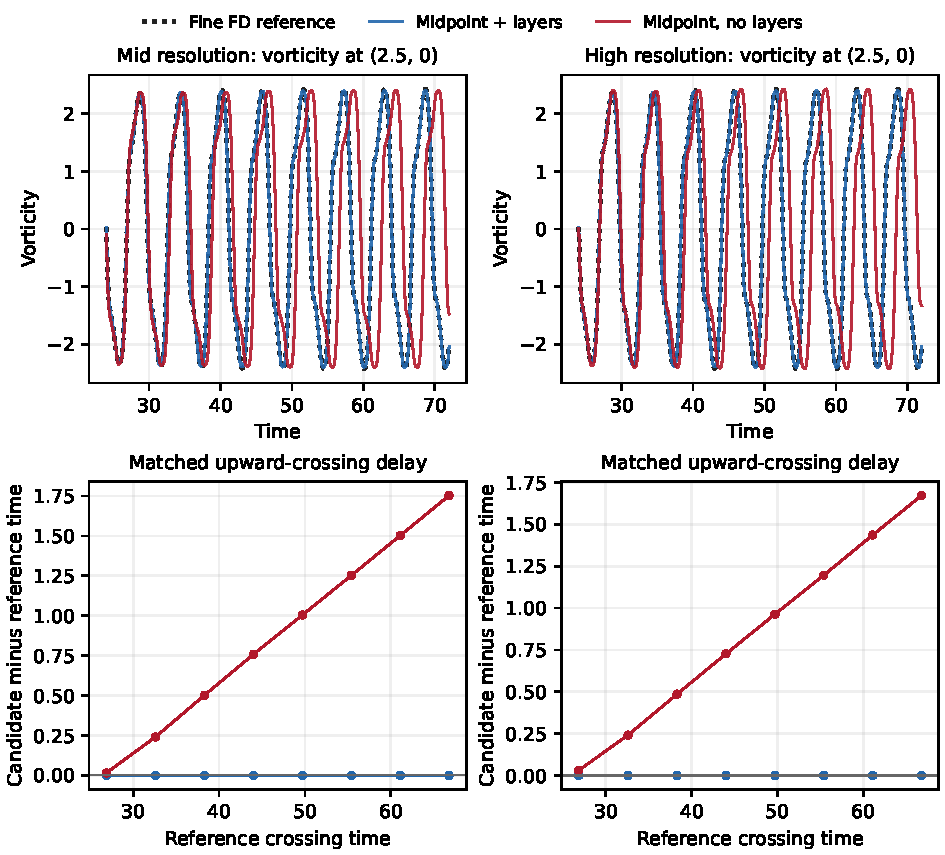
\includegraphics[width=\linewidth]{figures/review_phase_probes.pdf}
\caption{固定中点频率消融的原始时刻涡量信号及累计过零延迟。先将候选第一个相关过零事件与最近的初始参考事件配对，此后保持事件序号。下排仅在事件检测时去除线性趋势，没有平移任何轨迹或场误差评分。}
\label{fig:review-phase-probes}
\end{figure}
